Este fue un estudio monocéntrico doble-ciego controlado por placebo y de grupos paralelos y fue llevado a cabo en su totalidad en la Subdirección de Investigaciones Clínicas del Instituto Nacional de Psiquiatría Ramón de la Fuente Muñiz (INPRFM) en la Ciudad de México.
La investigación forma parte de un proyceto mayor financiado por CONACYT:
``Cambios en la estructura y conectividad funcional cerebrales relacionados a la mejoría clínica en pacientes con adicción a la cocaína después de un tratamiento con esitmulación magnética transcraneal'',
clave S0008-2015-2-260971, bajo la dirección del doctor Eduardo Garza Villarreal y aprobado por el Comité de Ética del INPFRM (CEI/C/070/2016).

\section{Muestra}
\begin{figure}[h!]
    \centering
    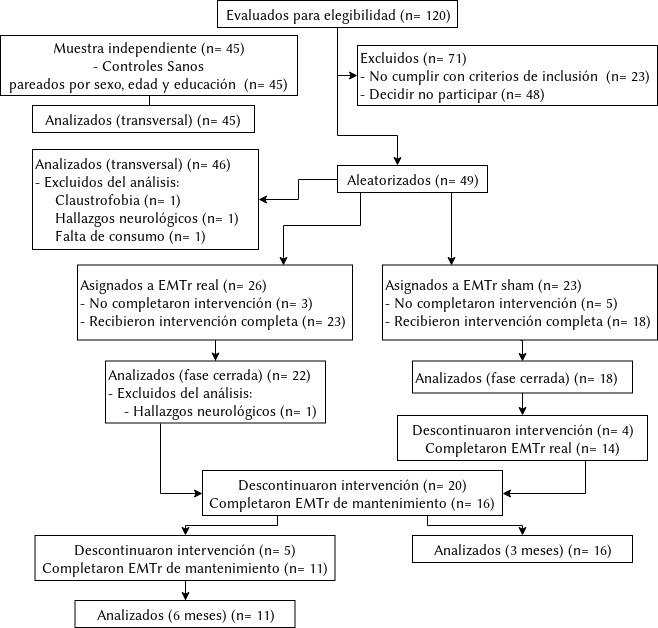
\includegraphics[width=\textwidth]{participantFlow}
    \caption{Diagrama de flujo de participantes}
    \label{fig:flow}
\end{figure}

Tanto pacientes de la clínica de adicciones del INPFRM como externos que cumplieran con el diagnóstico de dependencia de cocaína (F14.2x) del DSM 5 \parencite{APA2013} fueron reclutados para participar en el ensayo clínico.\par
XXX sujetos fueron asignados aleatoriamente a los distintos grupos de estimulación (Figura \ref{fig:Flow}).
Un grupo recibió estimulación sobre la corteza prefrontal dorsolateral izquierda y el otro, el protocolo sham de estimulación simulada sobre la misma área.
Una muestra de sujetos controles sanos pareados por edad, sexo y nivel de educación fue extraída de los datos de un estudio realizado con anterioridad en el INPFRM \parencite{Garza2017}.

\section{Criteros de selección}
Se siguieron los criterios de selección establecidos en el proyecto principal.
Estos fueron propuestos con la intención de disminuir la posibilidad de aparición de cualquier variable extraña y de seguir los lineamientos de seguridad tanto para la MRI como la EMTr.

\subsection{Criterios de inclusión}
Todos los participantes debían cumplir con los siguientes criterios para ser registrados en el estudio y ser asignados a uno de los grupos de investigación
\begin{enumerate*}[label=\emph{\alph*}), before=\unskip{: }, itemjoin={{; }}, itemjoin*={{, y }}]
    \item tener una edad mínima de 18 años y máxima de 50 años
    \item ser usuario de cocaína durante al menos dos  años, con un uso promedio actual mínimo de tres veces a la semana y periodos de abstinencia contínua menores a un mes durante el último año
    \item poseer un nivel de lectura de al menos 6to año de primaria
    \item tener la capacidad de dar un consentimiento informado válido
    \item ser diestro
    \item tener un índice de masa corporal menor o igual a 30;
    \item para las participantes del sexo femenino y en edad fértil, comprometerse a utilizar una forma médicamente aceptable\footnote{Píldora anticonceptiva, preparación hormonal, DIU o depósito (anillo, inyección, implante) y/o algún método anticonceptivo de barrera (diafragma, esponja, espermicida o condón).} de anticonceptivo y no quedar embarazada durante el estudio.
\end{enumerate*}

\subsection{Criterios de exclusión}
Los participantes fueron excluidos del estudio si presentaron cualquiera de las siguientes características
\begin{enumerate*}[label=\emph{\alph*}), before=\unskip{: }, itemjoin={{; }}, itemjoin*={{, e }}]
    \item antecedentes personales o familiartes de primer grado de cualquier trastorno neurológico, historia personal de neurocirugías previas o traumas craneoencefálicos que hayan producido pérdida de la conciencia
    \item tener alguno de los siguientes: marcapasos cardiáco, estimuladores neuronales, desfibriladores implantable, bomba de medicación implantada, líneas intracardiacas, implantes intracraneales (clips de aneurisma, derivaciones, estimuladores, implantes cocleares o electrodos) o cualquier objeto metálido dentro o cerca de la cabeza que no pueda ser retirado de forma segura
    \item esquirlas de metal o proyectiles metálicos en la cabeza o cuerpo
    \item uso actual de cualquier droga de investigación o de cualquier medicamento con acción proconvulsivante\footnote{Antidepresivos tricíclicos o neurolépticos que disminuyen el umbral convulsivo.}
    \item presión intracraneal aumentada
    \item historia de esquizofrenia, trastorno bipolar, manía o hipomanía
    \item historia de infarfo de miocardio, angina de pecho, insuficiencia cardiaca congestiva, miocardiopatía, eventos vasculares cerebrales o ataque isquémico transitorio, o cualquier afección cardiaca actualmente bajo atención médica
    \item en mujeres, tener un potencial reproductivo y no utilizar una forma aceptable de anticoncepción, estar embarazadas o en lactancia
    \item cualquier historia de convulsiones
    \item dependencia actual (criterios DSM-5) a cualquier sustancia distinta a la cocaína o nicotina
    \item claustrofobia
    \item historia de infección por VIH o positivo a prueba de anticuerpos del VIH
\end{enumerate*}

\subsection{Criterios de eliminación}
Los criterios para suspender la participación de los sujetos durante el estudio fueron
\begin{enumerate*}[label=\emph{\alph*}), before=\unskip{: }, itemjoin={{; }}, itemjoin*={{, y }}]
    \item expresar deseo de dejar de participar
    \item presentar hallazgos radiológicos anormales que ameriten mayor atención fuera del estudio
    \item aparición de síntomas psicóticos relacionados con el trastorno adictivo
    \item presencia de una elevación anormal de ánimo relacionada a la aplicación de la EMTr.
\end{enumerate*}

\section{Proceso del estudio}
\begin{figure}[h]
    \centering
    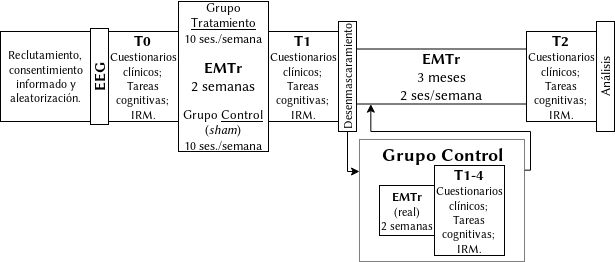
\includegraphics[width=\textwidth]{Des1}
    \caption{Linea de curso del tratamiento clínico de EMTr}
    \label{fig:txTMS}
\end{figure}

El estudio consiste en 4 etapas principales (Figura \ref{fig:txTMS}):
\begin{enumerate}[start=0,leftmargin=3\parindent,align=left,label=Etapa \arabic*:]
    \item Filtro de pacientes y etapa basal;
    \item Dos semanas de tratamiento aleatorizado;
    \item[Etapa 1-4:] Dos semanas de tratamiento real (grupo sham);
    \item Tres meses de tratamiento de mantenimiento.
    \item Seis meses de tratamiento de mantenimiento.
\end{enumerate}

\subsubsection{Etapa 0}
Los participantes fueron reclutados inter- y externamente entre aquellos que estuvieran interesados en un tratamiento para la dependencia a la cocaína.
Todos fueron entrevistados por un psiquiatra del instituto sobre los criterios de inclusión y exclusión.
En caso de ser admitidos al estudio, se les explicó completa y detalladamente las características principales del mismo y se les dió a firmar un consentimiento informado.
La asignación a grupos fue realizada por medio de un algoritmo aleatorizado por el director de la unidad y guardado en una memoria USB para cada sujeto que sería introcida directamente al resonador con tal de mantener el estado de doble-ciego.
La evaluación basal (T0) de los pacientes consistió en
\begin{enumerate*}[label=\emph{\alph*}), before=\unskip{: }, itemjoin={{; }}, itemjoin*={{, y }}]
    \item una entrevista clínica semi-estructurada aplicada por un psiquiatra
    \item una bateria de escalas clínicas aplicada por un psiquiatra
    \item una bateria de tareas cognitivas aplicadas por asistentes de investigación entrenados
    \item una prueba toxicológica de orina
    \item una corrida de MRI.
\end{enumerate*}
A todos los participantes se les aplicó un electroencefalograma para descartar cualquier actividad anómala que pudiera sugerir predisposición a un episodio convulsivo antes de iniciar con la fase de tratamiento.

\subsubsection{Etapa 1}
La primera fase de tratamiento consistió en 20 sesiones de EMTr real o sham, a lo largo de 10 días hábiles consecutivos. Cada sesión fue aplicada por un técnico entrenado en la administración de EMTr, quien tomó el umbral motor, ubicó la zona de estimulación y se encargo de aplicar los trenes de estimulación y supervisar posibles efectos adversos.
Los pacientes tuvieron un descanso de 30 minutos entre ambas sesiones.
Al finalizar, el técnico tomó un registro de cualquier molestia y se agendó la cita del siguiente día.\par
Terminando las 10 sesiones, los pacientes pasaron por otra evaluación (T1) clínica, de orina y MRI, antes de ser revelada su asignación de grupo.

\subsubsection{Etapa 1-4}
Para aquellos participantes que llevaron estimulación sham, se les ofreció continuar con un tratamiento de EMTr por otras 20 sesiones, con las mismas características que el grupo de tratamiento real. Una vez concluidas las dos semanas de la fase abierta, una tercera evaluación clínica, de orina y MRI (T1-4) fue realizada.

\subsubsection{Etapa 2}
Esta etapa consistió en la primera fase de sesiones semanales de mantenimiento. Cuando los pacientes terminaron con las 20 sesiones de tratamiento real, se les citó semanalmente para dos sesiones de mantenimiento de EMTr. Al completar los tres meses, los pacientes tuvieron otra evaluación clínica, de orina y MRI (T2).

\subsubsection{Etapa 3}
Se continuó el mantenimiento bajo las mismas condiciones hasta completar los seis meses y llevar a cabo una última evaluación clínica, de orina y MRI (T3).

\section{Instrumentos}
\subsection{Medidas de craving y recaída}
\begin{description}
    \item[CCQ-G] Cuestionario de Craving de la Cocaína, versión general (Cocaine Craving Questionnaire, General); escala que evalúa el deseo intenso hacia la droga de forma promedio en la última semana \parencite{Tiffany1993}.
    \item[CCQ-N] Cuestionario de Craving a la Cocaína, versión actual (Cocaine Craving Questionnaire, Now); escala que evalúa de forma presente el deseo intenso hacia la droga en el momento de aplicación \parencite{Tiffany1993}.
    \item[VAS] Escala Visual Análoga; escala visual análoga de \SI{100}{\milli\meter} utilizada para representar el \textit{craving} en el momento.
    \item[Línea de tiempo restrospectiva] Calendario de consumo como herramiento para medir el \emph{lapso} (por lo menos un evento de consumo con patrón diferente al basal) y \emph{relapso} (evento de consumo con el mismo patrón que el consumo basal).
\end{description}
\subsection{Medida de impulsividad}
\begin{description}
    \item[BIS-11] Escala de impulsividad de Barratt 11 (Barratt Impulsivity Scale 11); escala clínica que evalúa multidimensionalmente el índice de impulsividad \parencite{H.Patton1995,Salvo2013}.
\end{description}
\begin{enumerate}[label=Subescala \arabic*., left=3\parindent]
    \item Impulsividad atencional
    \item Impulsividad motora
    \item Impulsividad de no-planeación
\end{enumerate}

\section{Estimulación magnética transcraneal repetitiva (EMTr)}
\subsection{Localización de la corteza prefrontal dorsolateral}
El objetivo de la estimulación cortical será establecido tomando como base puntos de referencia craneales, utilizando la distancia teórica entre la región cortical objetivo y un punto en el cuero cabelludo determinado por EMT (procedimiento guiado funcionalmente) \parencite{Sparing2008}.
El área cortical motora izquierda fue el punto de referencia.
M1 fue determinada como la zona en donde hubiera una respuesta motora prominente en el dedo pulgar de la mano contralateral.
El umbral motor (MT) fue definido como la intensidad de estimulación menor que produjera una respuesta motora en al menos tres de cinco pulsos.
La localización de la corteza prefrontal dorsolateral fue \SI{5}{\centi\meter} anterior y \SI{2}{\centi\meter} lateral a M1 \parencite{Herwig2001a,Varnava2011a}.

\subsection{Estimulación real}
La EMTr fue aplicada ocon un estimulador rápido Magpro R-30 MagVenture (Medtronic, Dinamarca), equipado con una bobina MCF-P-B70 en forma de 8, de \SI{75}{\milli\meter} de diámetro interno en cada espiral, con enfriamiento estático y capacidad de estimulación sham. \par
El centro de la bobina fue colocado sobre la corteza prefrontal dorsolateral izquierda con el asa a \SI{45}{\degree} relativos a la linea media-sagital. \par
La estimulación se aplicó en dos sesiones de EMTr a alta frecuencia (\SI{5}{\hertz}) en un mismo día separadas por un intervalo inter-sesión de \SI{30}{\minute}.
Cada sesión consistió en 50 trenes de \SI{10}{\second} con un intervalo inter-tren de \SI{1}{\minute} a 100\% del umbral motor, dando un total de 5000 pulsos divididos en dos sesiones de \SI{58}{\minute} y de 2500 pulsos.

\subsection{Estimulación sham}
La estimulación sham fue dada con el mismo estimulador y parametros que la estimulación real, sin embargo, la bobina fue colocada en su posición sham donde el sonido es idéntico a la estimulación real, pero no dispara ningun pulso electromagnético.
A todos los sujetos durante las dos semanas de fase ciega se les colocó un electrodo en el músculo frontal sincronizado con el resonador on el fin de simular la sensación de la estimulación independientemente del grupo de tratamiento y mantener el doble-ciego.

\section{Imagen por resonancia magnética}
\subsection{Adquisición}
Tomamos la imagen por resonancia magnética con un resonador Philips Ingenia de \SI{3}{\tesla} (Philips, EEUU) y una antena de cráneo de 32 canales. La corrida consistió en una secuencia estructural T1w de alta definición, una secuencia EPI de fMRI en estado de reposo, una secuencia de difusión HARDI-DWI y una secuencia experimental FAST-DKI. Sin embargo, para la presente investigación, solo utilizamos las secuencias funcional y estructural.\par
Para la secuencia funcional, a los pacientes se les instruyó que se recostaran en el resonador moviéndose lo menos posible, que no pensaran en nada en específico y mantuvieran los ojos abiertos. Una cruz de fijación fue proyectada durante la secuncia funcional, pero no tenían que enfocarse en esta. \par
La fMRI fue tomada con una secuencia EPI (eco-planar) T2* con los siguientes parámetros
\begin{enumerate*}[label=\emph{\alph*}), before=\unskip{: }, itemjoin={{; }}, itemjoin*={{, y }}]
    \item TR = \SI{2}{\second}
    \item TE = \SI{30}{\milli\second}
    \item ángulo de inclinación de \SI{75}{\degree}
    \item 37 cortes de \SI{3.33}{\milli\meter} de grosor sin espacio entre corte
    \item FOV = \SI{240}{\milli\meter}
    \item matriz de \num{80x80}
    \item voxel de \SI[product-units=single]{3x3x3.33}{\milli\meter}.
\end{enumerate*}
Una secuencia \textit{fieldmap} fue tomada en dirección opuesta para el preprocesamiento.\par
La secuencia 3D de alta resolución T1w fue adquirida con los siguientes parámetros
\begin{enumerate*}[label=\emph{\alph*}), before=\unskip{: }, itemjoin={{; }}, itemjoin*={{, y }}]
    \item TR = \SI{7}{\milli\second}
    \item TE = \SI{3.5}{\milli\second}
    \item ángulo de inclinación de \SI{8}{\degree}
    \item 180 cortes de \SI{1}{\milli\meter} de grosor sin espacio entre corte
    \item FOV = \SI{240}{\milli\meter}
    \item matriz de \num{240x240}
    \item voxel de \SI[product-units=single]{1}{\milli\meter\cubed}.
\end{enumerate*}

\subsection{Manejo de datos}
Los datos de imagen fueron extraídos del formato \texttt{DICOM}, transformados a \texttt{NIfTI} y organizados en \texttt{BIDS} \parencite{Gorgolewski2016}.
La calidad de los datos fue evaluada con \texttt{MRIQC} \parencite{Esteban2017} para evaluar posibles artefactos de señal y/o movimiento. \par
as imagenes fueron preprocesadas utilizando \texttt{FMRIPREP v1.4.1} \parencite{Esteban2019}, una herramienta basada en \texttt{Nipype} \parencite{Gorgolewski2011}.
Cada volumen de las imagenes T1w fue corregido por INU (no-uniformidad en intensidad) usando \texttt{N4BiasFieldCorrection v2.1.0} \parencite{Tustison2010} y se les removió el cráneo con \texttt{antsBrainExtraction.sh v2.1.0} (con la plantilla OASIS).
La normalización espacial a la plantilla ICBM 152 asimétrica no-lineal versión 2009c \parencite{Fonov2009} fue realizada por medio de un registro no-lineal con \texttt{antsRegistration} de \texttt{ANTs v2.1.0} \parencite{Avants2007}, usando versiones sin cráneo tanto del volumen T1w como de la plantilla.
La segmentación del tejido cerebral del líquido cefaloraquídeo (LCR), sustancia blanca (WM) y gris (GM) fue realizada en la imagen T1w sin cráneo usando \texttt{fast} de \texttt{FSL v.5.0.9} \parencite{Zhang2001}.\par
Los datos funcionales fueron corregidos en el tiempo de corte usando \texttt{3dTshift} de \texttt{AFNI v16.2.07} \parencite{Cox1996} y corregidos por movimiento con \texttt{mcflirt} (\texttt{FSL v5.0.9} \parencite{Jenkinson2002}.
Esto fue seguido por un co-registro al volumen T1w correspondiente usando un registro basado-en-límites \parencite{Greve2009} con seis grados de libertad, usando \texttt{bbregister} (\texttt{FreeSurfer v6.0.1}).

















